\documentclass[fontsize=8pt]{memoir} % use article if you want to use the old IPAD latex 
% otherwise use memoir class
\usepackage[utf8]{inputenc}
\usepackage[paperwidth=9cm, paperheight=11.5cm, top=0.5cm, left=0.5cm, right=0.5cm, bottom=0.5cm]{geometry}
\usepackage{graphicx}
\usepackage{url}
\usepackage{minted}
\usepackage{listings}
\usepackage{cite}


% remove this if you wanted to use the old IPAD latex
% just added
\usepackage{tikz, blindtext}

\makechapterstyle{box}{
  \renewcommand*{\printchaptername}{}
  \renewcommand*{\chapnumfont}{\normalfont\sffamily\huge\bfseries}
  \renewcommand*{\printchapternum}{
    \flushright
    \begin{tikzpicture}
      \draw[fill,color=black] (0,0) rectangle (2cm,2cm);
      \draw[color=white] (1cm,1cm) node { \chapnumfont\thechapter };
    \end{tikzpicture}
  }
  \renewcommand*{\chaptitlefont}{\normalfont\sffamily\Huge\bfseries}
  \renewcommand*{\printchaptertitle}[1]{\flushright\chaptitlefont##1}
}

% end of just added


% fonts

%%\usepackage[scaled]{helvet}
%%\usepackage[defaultsans]{droidsans}
%%\usepackage[scaled]{libertine} 
%%\usepackage{lmodern} 

%% \usepackage[T1]{fontenc}
%% \usepackage{berasans}

% \usepackage[default]{gfsneohellenic}
% \usepackage[LGR,T1]{fontenc}

% \usepackage[light,math]{kurier}
% \usepackage[T1]{fontenc}

% \usepackage[math]{iwona}
% \usepackage[T1]{fontenc}

\usepackage{cmbright}
\usepackage[T1]{fontenc}

\renewcommand*\familydefault{\sfdefault}

% end of fonts

% uncomment this if you wanted to use the old IPAD latex
% \newcommand{\chapter}[2]{\begin{center}\section*{#1}\textbf{#2}\end{center}}

\usepackage{todo}
%Begin Decorative packages
\usepackage{type1cm}
\usepackage{lettrine}
\usepackage{fourier-orns}

\renewcommand{\pfbreakdisplay}{%
\decofourright\quad\decofourright\quad\decofourright
}

\usepackage{natbib}

%End decorative packages

\frenchspacing
\sloppy
\pagestyle{empty}

% remove this if you wanted to use the old IPAD latex
\chapterstyle{box}
\begin{document}

\title{\uppercase{SnipR}: Complementing Code Search with Code Retargeting Capabilities}
\author{by Huascar A. Sanchez}

\date{}
\maketitle
%\newpage
%\noindent
%[Disclaimer: For sake of convenience, I am temporarily using this latex template to improve the readability and accessibility of this document. Page margins and font size are increased, etc., giving the illusion of long sections. This template works perfectly in cases where you want to review this document from portable devices, such as the iPhone, iPad, Kindle, Android Tablet, etc.]
% \newpage

\chapter{Introduction}{}
\label{sec:intro}

\lettrine[lraise=0.1, nindent=0em, slope=-.5em]{T} {HE RECENT RISE} of Internet-scale code search engines---e.g., Sourcerer~\cite{Bajracharya:2006vn}, Portfolio~\cite{McMillan:2011wq}, SEAHAWK's Crawley~\cite{Bacchelli:2012dl}, Koders~\footnote{\url{http://www.koders.com}}---has catapulted search-driven development from backwater to ubiquity, and given rise to an active research community focused on this phenomena~\cite{Bajracharya:2009fj, Bajracharya:2010iy, Bajracharya:2011kw}. The increased prevalence of such engines has given search-driven development more diverse sources of information---e.g., from open sourced code to code snippets from StackOverflow~\footnote{\url{http://www.stackoverflow.com}} on programming questions---and a more open platform---the Internet~\cite{GallardoValencia:2009gr, GallardoValencia:2010ij, Ying:2012tr}. This new condition has enabled developers to build applications opportunistically by iteratively finding, combining, and reusing online source code~\cite{Brandt:2008wi, Brandt:2009jb, Ying:2012tr}. However, this opportunistic way of building applications is not easy because searched sources are large, in most cases unsuitable, and quite often unrelated~\cite{GallardoValencia:2009gr}. Consequently, if one wants to establish search-driven development as a best practice, then one has to minimize the time involved in deciding the best search result(s) to reuse.

Previously published work has tried to tackle the above problem from different directions. Two of these directions are the most popular. One direction focuses entirely on enhancing search technology~\cite{Bajracharya:2010um, Gysin:2010kt, Mandelin:2005uj, McMillan:2011cm, McMillan:2012dj}, while the other direction focuses on coupling Web search and community-based knowledge with IDEs~\cite{Bacchelli:2012dl, Brandt:2010tp, Hartmann:2010hx, Hoffmann:2007wo, Wightman:2012gc}. Although these directions focus on addressing the trustability and relevance of search results, none of them adequately address the \emph{suitability} of these results. In other words, developers are given no guidance as to which result may be a best fit for their code in progress, beyond the existing ranking values. Precisely, developers still have to \emph{manually} mine and try all these ranked results before they could possibly realize their usefulness---or uselessness. This limitation is one of the main reasons why search-driven development is so cumbersome, and ultimately can be a drain on one of the most precious resources in software development: time.

An increasingly familiar example of search-driven development arises when modifying a program to support a particular set of functionality. Sometimes, the task is to reuse external third-party libraries, or to support algorithms with specific performance characteristics. Other times, a developer may want to support a feature implemented by code with a conflicting API\footnote{Application Programming Interface (API)}. A good example would be adapting a sentiment analysis tool (that uses the Twitter API) to use the Facebook API. This type of tool permits the classification of opinions in text (e.g., status updates in Twitter) into categories like ``positive'' or ``negative.'' 

The increased prevalence of open source software and code search tools makes it simpler to find large sets of relevant examples~\cite{Reiss:2009fu}. As for the above sentiment analysis tool, one could find around fifty platform-specific Facebook libraries and a few dozens general-purpose Facebook libraries on Github\footnote{\url{http://www.github.com}}, each with unique differences and similarities. Tool support for \emph{anticipating} whether any source code found in those libraries is a best fit for one's code is basically non-existent, making any integration tasks heavyweight, tedious, and error-prone. 

%Both Facebook and Twitter are popular services with different purpose and functionality, and yet they share a common feature: text-based status updates. This suggests that there is an exploitable correspondence between the ``status updates'' source code of the two services' APIs. Due to these services' popularity in the open source world\footnote{Search for Twitter or Facebook at \url{www.github.com}.}, it is common for one to rely on the proliferation of open source software and the availability of code search tools to find large sets of relevant examples~\cite{Reiss2009}. These are examples that could potentially help changed the sentiment analysis tool to use the Facebook API. Even if one were to overlook these dependencies, the absence of tool support for \emph{anticipating} the usefulness of retrieved examples makes retargeting\footnote{Retargeting is the process of altering source code to fit an alternate context.} tasks heavyweight, tedious, and error-prone. %All these factors combined imply that code search all by itself doesn't solve the whole problem.%%In the context of modifying the bullying detection program, the absence of such tool support could lead to the developer going beyond the time allocated for the task or not finishing the task at all. This is augmented, in part, by the %developer constantly switching \emph{back and forth} between results evaluation and further searches. 

Obviously, code search all by itself doesn't solve the whole problem. In fact, code-only searching misses out on certain human abilities that are important in search-driven development, such as the ability to quickly identify better results among a myriad of retrieved examples, to highlight relevant elements (e.g., variable names), to demarcate feasible regions of code, and to transform results into code that resembles what existed only in the human mind. Do note there are systems, such as~\cite{Bajracharya:2010um, Gysin:2010kt, Hartmann:2010hx, McMillan:2012dj, Sawadsky:2011eh, Wightman:2012gc} that are starting to address these issues; each with unique strengths and weaknesses. However, tool support for anticipating the usefulness of any potentially suitable search result based on the above abilities is inchoate, leaving developers to perform the retargeting\footnote{Retargeting is the process of altering a source code to fit an alternate context} the old fashioned way. The consequent effect of these limitations is a surprisingly significant reduction of productivity~\cite{Cypher:2010ub, Gysin:2010kt}.

Given this hit on productivity, I propose a radically new approach in search-oriented architecture, called \emph{Snippet Retargeting Model} or simply \emph{SnipR}. This approach complements code search by supercharging it with code retargeting capabilities. The intent of these capabilities is to expedite the process of determining if a source code is a best fit; i.e., suitable. These capabilities are embedded within \emph{query processing} in order to automatically modify retrieved source code. Each query issued by a developer is interpreted by the query engine not only as a request for a particular result set, but also as a command to retarget relevant bodies of code in that set; e.g., modify a retrieved example---in place---to use an alternative API. With this in mind, the usefulness of retrieved source code can now be anticipated by applying, within query operators, code mappings to the retrieved source code and to later and similar examples. A code mapping is a semantic-preserving code transformation learned from code examples (i.e., search results) and encapsulated in a representation that could be accessed algorithmically. They specify how two or more code examples correspond, and when applied to a base example, it produces a variation containing the changes specified by the mapping. This type of code retargeting is performed in place, without requiring to leave the search interface. As for the sentiment analysis tool, \emph{SnipR} would allow an iterative approach for changing the tool's code from using the Twitter API to using the Facebook API. One would inspect the result set; demarcate the code block (s) to be transitioned; infer corresponding mappings; apply these mappings; and evaluate the resulting examples. At this point, one would rely on the suitability of these candidates to identify the next course of action. 

\begin{figure}[!ht]
    \centering
    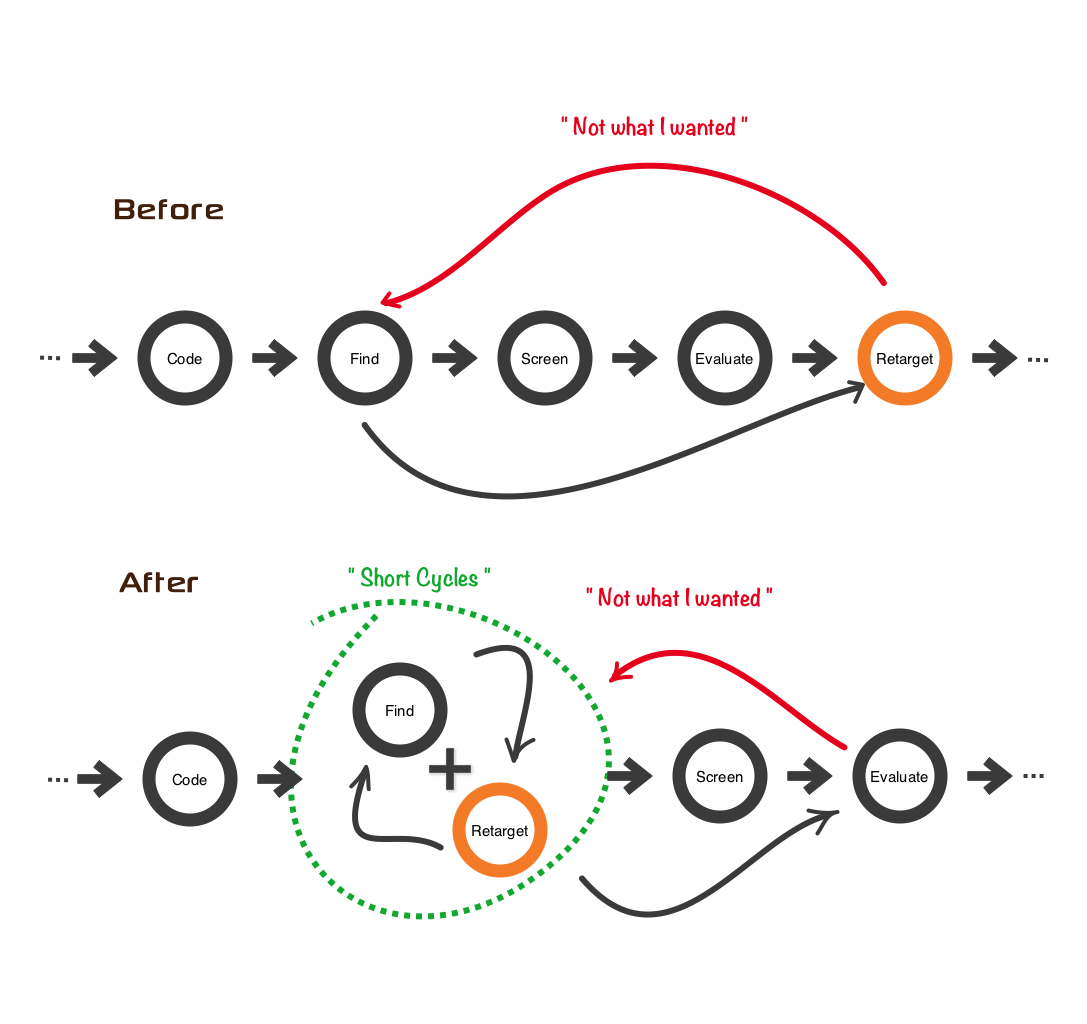
\includegraphics[width=\textwidth,height=0.8\textheight,keepaspectratio]{images/searchprocess}
    \caption{Search Process before and after \emph{SnipR}}
    \label{fig:retargeting}
\end{figure}

Figure~\ref{fig:retargeting} illustrates the search process before and after \emph{SnipR}. A pre--\emph{SnipR} scenario requires effort from the developer to find and select the most promising examples (i.e., screening), and to evaluate each one of them before eventually consuming them (e.g., done with integration) after a series of code modifications done directly from the IDE (i.e., retargeting). If the resulting code is not what the developer wanted, then the developer will restart the search process. In a post--\emph{SnipR} scenario, the developer engages in virtuous loop where the developer finds only the promising code that can be retargeted. This minimizes the number of iterations in the search process, since the screening and evaluation steps are only dealing with best choices---choices that would be easier to consume at the IDE.

In retrospect, if the time required to determine the most suitable results is minimized by retargeting, then the effort of integrating these search results is also minimized. If retargeting is unsuccessful, then the developer will continue searching for more examples and retarget as needed. Overall, \emph{SnipR} will allow requests for results and commands\footnote{The everyday search box would be enhanced with command line power; e.g., code manipulation commands.} to be intermixed---or used separately---by the developer to explore potential modifications of example code (See post--\emph{SnipR} scenario in Figure~\ref{fig:retargeting}). This offers two important advantages. If the developer retargets the source in advance, then the analysis results (i.e., evaluation) of retargeted examples are available immediately, which saves valuable human time searching for appropriate example code. If the developer is choosing what example code to retarget, then the analysis results can inform the decision, pointing the developer to the best choice. This is an attractive proposition and very different to the direction taken by the status quo. It is attractive because one can figure out as early as possible if an example code is appropriate or not. It is different because one can do this without requiring to leave the search interface.
% This proposed approach suggests an environment where human and search engine help each other out and accept the challenge of retargeting code on the spot.  

This work anticipates the following technical and theoretical contributions:

\begin{itemize}
\item I'd provide a command line language for retargeting source code directly from a search interface. 
\item I'd present the algorithms that infer code mappings from example code and the new 
    retargeting operators well suited for manipulating example code; i.e., applying created mappings.
\item I'd present the first search-oriented architecture---based on \emph{SnipR}---in the context of 
    better code search engines. 
\item I'd report on my implementation of this architecture on top of Sourcerer\cite{Bajracharya:2006vn}, showing that this architecture is easy to implement.
\item I'd evaluate this architecture and discuss generated results.
\item I'd provide an evaluation of the efficiency of the \emph{SnipR} approach versus existing approaches. 
\end{itemize}

\fancybreak{\pfbreakdisplay}

\section{Research Questions}
\label{sec:questions}

An essential part of knowing what kind of search-driven tools could help developers find the right examples to reuse is knowing precisely why search-driven development is so difficult. I would examine this question by answering the following guiding questions: 

\begin{itemize}
	
	\item[RQ1] What kind of \uppercase{SnipR} commands could be invoked directly from the search 
	box? 
	
	The aim is to design a set of retargeting commands that could be invoked by developers from the 
	search box, without losing any sight of their current search goal. This design should balance 
	two inter-related principles: simplicity and flexibility. For simplicity, SNIPR will provide 
	most of the mechanisms for expression and control of changes that could be made to modules 
	(methods that implement an API). This involves discovering the fundamental concepts of 
	retargeting modules, to extract them from their various reincarnations, and to present them in a 
	pure and distilled form. This form will be inspired by the syntax of the Io programming 
	language. For flexibility, a simple language for combining, and executing code retargeting 
	commands will be developed. This language's goal is to extend \uppercase{SnipR}'s availability 
	functionality. To evaluate simplicity, a user study and a survey will be performed. For 
	flexibility, the statistics on the use and execution effort for supporting and using different 
	commands will be reported.
		
	% That is, it should resemble the language used by developers when 
	% 	modifying source code, and allow a reasonable set of code changes to be expressed. By applying a 
	% 	simple but well principled rule, I would be able to decide when I have completed this question: This question is 
	% 	complete when I have stopped finding reasons to change any of the already defined commands.
	% 	
	% \item[RQ1] How does \emph{SnipR} compare to existing search-driven development 
	% 	systems~\cite{Bajracharya:2010um, Gysin:2010kt, Hartmann:2010hx, McMillan:2012dj, Sawadsky:2011eh, Wightman:2012gc} and are there any decisive factors in deciding on the approach or 
	% 	system to be used for search-driven development? 
	% 	
	% 		
	% 	I will show \emph{SnipR} is less a competitor to any of the above referenced systems and more 
	% 	of a platform. It is an effective way to improve the search for suitable 
	% 	examples, but any number of other development tools can come into play after 
	% 	the retargeting of the first few examples.  
	% 	%\emph{SnipR} will target a situation where the users don't know what they want until 
	% 	%they see it. There's no prior knowledge about the usefulness or uselessness of those 
	% 	%examples, and there is limited time and resources.
	% 	
	\item[RQ2] How expensive is it to retarget (part of) found source code each time?
	
	This question is about the performance (in terms of computational throughput) of the code 
	retargeting algorithms. In other words, this is about how long it will take the code retargeting 
	algorithms to apply the appropriate code mappings to any found source code. Code retargeting is 
	an operation that can operate on a single result or an entire result set. Therefore, this 
	operation requires that those cases where code mappings can be learned and/or applied are 
	carefully identified. This will prevent any unnecessary work from happening as matched code 
	examples are being returned by the query engine. To evaluate the performance of this algorithms, 
	a set of microbenchmarks will be implemented, and the obtained statistics reported.
	
	% Per Jim's comment on Sunday Oct 28, 2012 
	% \item[RQ2] What is the impact on programming time when retargeting is done at the 
	% integrated development environment versus when it is done at the search interface?  
	% 
	% Significant amount of time is lost when developers must move retrieved code from one 
	% environment to another. The screening and changing of the retrieved code at the 
	% search interface would minimize any back and forth movement between results 
	% evaluation and further searches.
	
	\item[RQ3] Where does \uppercase{SnipR} belong within the query processing step of any 
	modern code search engine?
	
	The answer to this question will be based on a working system for code search, such as 
	Sourcerer\cite{Bajracharya:2006vn} Internet-scale code search engine. This system will 
	be updated with \uppercase{SnipR}. Then, this work will rely on any experimentation performed 
	on the updated system to answer this question. 
	% 
	% \item[RQ3] Will productivity time increase when using SnipR versus not using SnipR?
	% 
	% Retargeting time is directly linked to integration time. If integration time goes 
	% down, then productivity time goes up. Since SnipR is trying to minimize 
	% integration time, then productivity is likely to increase.
	
	% \item[RQ4] How does the performance---in terms of the time to perform a more complete 
	% code search task---of a system using SnipR compare to systems where SnipR is not 
	% available?
	% 
	% \item[RQ4] How does the performance---in terms of the time needed to perform a more complete 
	% code search task---of the SnipR approach compare to the current approaches of code search? 
	
	\item[RQ4] How does the time needed to perform a more complete code search task of the 
	\uppercase{SnipR} approach compare to the current approaches of code search? 
	
	If the developer is retargeting the source in advance, then the evaluation results of 
	retargeted examples are available immediately (See \uppercase{SnipR} scenario in 
	Figure~\ref{fig:retargeting}). This immediate feedback saves valuable time searching for an 
	appropriate example code. As a result, by getting immediate feedback, the developer gets the 
	work done more quickly. This will hold true only if \uppercase{SnipR}'s retargeting operations 
	are efficient, which will be demonstrated by answering RQ2.
	
	% 
	%  
	% \item[RQ4] Will there be a productivity boost when using \emph{SnipR} versus not using \emph{SnipR}?
	% 
	% Retargeting in advance is directly linked to minimizing integration time. If integration time goes 
	% down, then productivity---the time required to write a fixed amount of code---goes up. Since the 
	% retarget code produced by \emph{SnipR} is the best fit, then the integration of such code is faster than the 
	% integration of less suitable code; i.e., code that relies only on ranking values. Consequently, I anticipate a 
	% boost in productivity.
		
	% \item[RQ4] Would the very way code manipulation is piggy-backed to query processing 
	% and advised by users' queries lead to a successful code integration?
	% 
	% If the most suitable results are found by retargeting, then the odds of code 
	% integration success are increased. By validating the SnipR approach 
	% and results in practice, I would be able to confirm whether the retargeted code 
	% produced by SnipR was successfully integrated.
\end{itemize}

All the work proposed in this document is motivated by a grander vision of where the next generation of programming practices and behaviors involving code search could take us. The time is ripe to change the role of code search as a development tool from a mere supporting role to a starring role.
\fancybreak{\pfbreakdisplay}

\section{Outline}
\label{sec:outline}

The rest of this document is structured as follows. In Chapter 2, I discuss related work.
Once the related is covered, I present the foundations of the Snippet Retargeting Approach in Chapter 3, 4, and 5. Chapter 3 describes the policy behind \uppercase{SnipR}. In Chapter 4, I describe the learning algorithm for building code mappings from code examples. This chapter also describes two procedures needed to set up \uppercase{SnipR}. In Chapter 5, I present Twist, a language for interacting with search results, and combining
and executing code retargeting operations. In Chapter 6, the proposed solutions, including the evaluation, and the work timeline are presented. Finally, Chapter 7 concludes the proposal.
\chapter{Related Work}{}
\label{sec:related}

\lettrine[lraise=0.1, nindent=0em, slope=-.5em]{S} {NIPR IS RELATED TO} prior work in three areas: example-centric programming; better code search systems; and systems for transitioning code to alternate contexts and/or APIs.

\fancybreak{\pfbreakdisplay}

\subsection{Finding Suitable Examples}
\label{sec:codesearch}

Many systems have been built to aid programmers with finding trustable and relevant example code. This includes systems that have gone on to include communal input or knowledge collaboration to suggest solutions to problems in the programmers' code. These systems differ from \emph{SnipR} in focus and approach. Instead of enabling programmers to examine---by retargeting in advance---whether a searched source is really suitable for their code in progress, these systems simply return many ranked results that programmers have to manually combine and retarget to discover if an example code is a best fit. 

For example, Brandt’s Blueprint system~\cite{Brandt:2010tp} couples Web search with development environments. Assieme~\cite{Hoffmann:2007wo} combines documentation search results with code snippets of the relevant functions currently in use. Stylos's Mica system~\cite{Stylos:2006gu} integrates search for documentation and example source code. Hartmann's HyperSource system~\cite{Hartmann:2011ii} associates browsing histories with source code edits. Hartmann's HelpMeOut system~\cite{Hartmann:2010hx} aids the debugging of code-related error messages by suggesting solutions that peers have applied in the past. McMillan's Source Code Recommender systems~\cite{McMillan:2012dj} combines mining written code specifications and open sourced code to recommend source code modules relevant to the application under development.
% dont trust me just because I am telling u to do it. E.g., dont trust this code is relevant just because there is a score that tells u that.

\fancybreak{\pfbreakdisplay}

\subsection{Code Search Engines}
\label{sec:searchengines}

In recent years many search engines for source code have appeared. The basic idea of such engines is to let developers search for example code and to present them results for their query. These engines use either keywords, unit tests, or semantic information to find large sets of relevant example code. Working examples of new functionality and solutions to problems in the developers’ code are now just one search away. This easy access to such an amazing treasure of trove code clearly has value; however, it has also significant limitations as a platform. These engines give developers no guidance as to which result may be a best fit for the developers' code in progress, beyond the existing ranking values. As for how they differ from \emph{SnipR}, one could see \emph{SnipR} as complementary to such research in code-centric engines. SnipR gives these engines a tool to predetermine if a source code is a best fit; i.e., suitable. Indeed, \emph{SnipR} is less a competitor to any of the above engines and more of a platform. It is a way to improve the search for suitable example code, but any number of other development tools can come into play after the retargeting of a few searched sources. 
         
Better code search engines, e.g., Sourcerer~\cite{Bajracharya:2006vn}, and Merobase~\cite{Hummel:eq}, provide ways of structured code search. They are accessible through IDEs---e.g., Eclipse---through plug-ins. These plug-ins allow developers to write unit tests, which in turn expands queries to find relevant classes and methods~\cite{Hummel:eq}. S$^{6}$ project\cite{Reiss:2009fu}, Code Genie~\cite{LazzariniLemos:2007jh}, Code Conjurer~\cite{Hummel:eq}, and Stolee's semantic searcher~\cite{Stolee:2012wp} focus on lowering the barrier for software reuse by using either a combination of meaningful specifications over source code or unit tests to search for relevant example code. McMillan's Portfolio~\cite{McMillan:2011cm, McMillan:2011wq} uses a combination of natural language processing (NLP), indexing techniques with PageRank and spreading activation network (SAN), while Prospector~\cite{Mandelin:2005uj} uses input and output types, etc.

\fancybreak{\pfbreakdisplay}

\subsection{Retargeting Source Code}
\label{sec:retargetingcode}



\chapter{\uppercase{SnipR} Fundamentals}{}
\label{sec:fundamentals}

% \fancybreak{\pfbreakdisplay}

\lettrine[lraise=0.1, nindent=0em, slope=-.5em]{T} {HIS CHAPTER} sets the stage for the complete description of the \uppercase{SnipR} in the next sections.

\section{Eager vs. Lazy Code Retargeting}
\label{sec:eagervslazy}

\uppercase{SnipR} builds on an eager code retargeting policy, a policy that is executed from the search interface. Below, this policy and its opposite---a lazy code retargeting policy, a policy that is executed at the IDE---are described.

\subsection{Eager Retargeting}

Eager retargeting is the policy of continually making code changes on one or more results, and feeding any suitability scrutiny on the outcome back into the search process\footnote{A rapid experimentation of example code}. A process that has such a policy operates under two assumptions:

\begin{enumerate}
	\item Code retargeting is a \emph{cheap}---efficient---operation, and
	\item Code retargeting ought to be done often
\end{enumerate}

Code retargeting ought to be done often in dynamic and exploratory scenarios---i.e., when the developer is working in an unfamiliar domain~\cite{Brandt:2009ew}. In such a scenario the type and number of example code may quickly change as further searches are performed. Also, if one wants to assure a rapid understanding of unfamiliar found code~\cite{Brandt:2009ew}, then it helps to frequently retarget any results to get a better picture of the result's suitability.

This policy accounts for the fact that it may not be possible to completely and safely perform code retargeting on certain snippets. In this case, the retargeting operation will result in an error. Therefore, we can hypothesize that if changes such as renaming functions or parameters, adding or removing arguments, or reorganizing structures cannot be applied, then the cognitive distance of the snippet's abstractions is high and the pay-off for reusing it is relatively small. Consequently, it can be safely discarded from the list of results to be screened by the developer.    

The expected advantages of eager retargeting are:

\begin{enumerate}
	\item The example code is more likely to match what the end user had in mind.
	\item The end user can have more confidence sooner that the picked examples were the right ones.
\end{enumerate}


\fancybreak{\pfbreakdisplay}

\subsection{Lazy Retargeting}

Lazy retargeting is the policy of only making code changes on a result at the point of integration. Under this policy, there is no guarantee---beyond relative ranking values---of the result's suitability. A process that has such a policy operates under two assumptions:

\begin{enumerate}
	\item Code retargeting is an \emph{expensive} operation, and
	\item Code retargeting ought to be done at the point of integration
\end{enumerate}

A process that has such a policy assumes code retargeting is a costly operation~\cite{Brandt:2009ew, Wightman:2012gc}. This is based on the observation that---at the point of integration---unrelated and/or unsuitable results require many more code changes than suitable results.

\fancybreak{\pfbreakdisplay}

\subsection{Reasoning about these two policies}

Intuitively, one needs to figure out whether an eager code retargeting policy leads to a \emph{cheaper} and thus \emph{faster} code search process than its opposite. 

One could model the notion of ``cost'' to retarget code examples with the following components:

\begin{enumerate}
	\item Code understanding
	\item Code modification
	\item Code disturbance
\end{enumerate}
 
The code understanding effort takes into account the time needed to carry out program comprehension actions, such as locating the snippet, doing content analysis, screening snippets. This effort is denoted by $U_{s}$, which is defined as the average effort required before starting the actual retargeting actions:

Code modification efforts represents the cost of changing the necessary tokens in a snippet. For a sequence of tokens `a', let $\alpha^{+}(a)$ and $\alpha^{-}(a)$ denote the cost of adding changes to ``a'' and removing those changes from ``a'' respectively. This term is formulated as: 

\begin{equation}
	\alpha(S_{1}, S_{2}) = C_{s} \times (\sum_{a \in S_2 - S_1}\alpha^{+}(a) + \sum_{a \in S_1 - S_2}\alpha^{-}(a))
	\label{costmodification}
\end{equation} where $C_{s}$ is the average estimated time for one generic snippet change performed by the developer.

Code disturbance expresses the cost of tinkering\cite{Jadud:2006ir} when developers face a problematic situation. It is assumed that code disturbance is proportional to the amount of interruptions---e.g., unpredictable errors---experienced by a developer during retargeting and how long each interruption takes as a snippet varies. This term is formulated as:

\begin{equation}
	\epsilon(S_{i}) = T_{s} \times Interruption(S_i)
	\label{costmodification}
\end{equation} where $T_{s}$ is the average estimated time an interruption takes, $S_i$ the snippet being modified, and $Interruption(S_i)$ the number of interruptions experienced when changing a snippet $S_i$. 

Therefore, the overall retargeting cost is defined as:

\begin{equation}
	cost(S_1, ..., S_n) = U_s + (\sum_{i=1}^{n}(\alpha(S_{i-1}, S_{i}) + \epsilon(S_{i})))
	\label{totalWork}
\end{equation} where $S_1, ..., S_n$ are different snippet variations that can be derived from retargeting actions, and $S_0$ is the initial snippet.   

From the above model, one can assume that the \emph{winner} policy is the one with the smallest total cost.

Eager retargeting assumes a low cost. This is based on the observation that unsuitable results---i.e., results that cannot be retargeted---are excluded more often\footnote{i.e., the search space is reduced.}, leaving the developer only suitable choices to handle; choices that are retargetable and help reduce the cognitive distance\cite{Krueger:1992wf}, experienced by developers, to understand how to use them. Obviously, this will lead to a low disturbance and thus to a low total cost.  

In contrast, as it has been already suggested in previous work~\cite{Brandt:2009ew, Wightman:2012gc}, a lazy retargeting policy assumes a high cost. Under this policy, it is common for one to look at each promising result (suitable or unsuitable) in its entirety\footnote{all the way to try to retarget each individual result at the IDE.}---usually one by one. If the retargeting of such result is unsuccessful, then the developer will try to explore the problem and then try all possible ways he/she can correct the problem. Not only this could lead to more frequent disturbances, more code changes and thus to a high total cost, but also to a sluggish searching interaction~\cite{Gray:2000im}.

Since the major ``cost'' of each policy is directly connected to the time spent by the developer searching for suitable code, a policy leading to a \emph{cheaper} code search process leads also to a \emph{faster} code search process.

% 
% \section{What rules should guide the Retargeting of found code?}
% \label{sec:sniprrules}
% 
% \uppercase{SnipR} models code searching as a short cycle of alternating query, screen, and retarget phases: found code is retargeted with commands issued just following to the displaying of a result set or prior to issuing a query (Figure). This model is operationalized using a state machine (Figure): during browsing, reported results are added to a queue; when the user .    
% 
% when the user edits code, all pages in the queue are assigned to new characters. 


\section{How to start developing with \uppercase{SnipR}}
\label{sec:sniprscenario}

A scenario will be given to help introduce the main interaction techniques. \uppercase{SnipR} offers two choices for interacting with code-centric sites: to issue queries and retargeting operations separately, or to intermix queries and retargeting operations. For sake of clarity, this section will focus on the former.

Olivia is an amateur developer and open source evangelist who frequently practice search-driven development at her workplace. Olivia would like to transition a sentiment analysis tool (that uses the Twitter API) to use the Facebook API. The updated tool should handle the sentiment classification of status updates in Facebook. She wants status updates to be classified dynamically. She is familiar with Java and has some Machine Learning experience, but does not consider herself an expert developer.

Olivia starts by opening Twist---a \uppercase{SnipR}-aware snippet-centric search engine she frequently visits for discovering open source libraries. This engine spans large sets of open source projects; mostly indexed from a variety of project hosting sites, such as Github, and Google code. Olivia interacts with Twist by using Twist's own language (also called Twist). This language allows Olivia to use queries and/or code retargeting operations to do code searching. The design of this language will be described in Chapter~\ref{chap:twist}. Figure~\ref{fig:twist} shows Twist's Web interface. 

\begin{figure}[!ht]
    \centering
    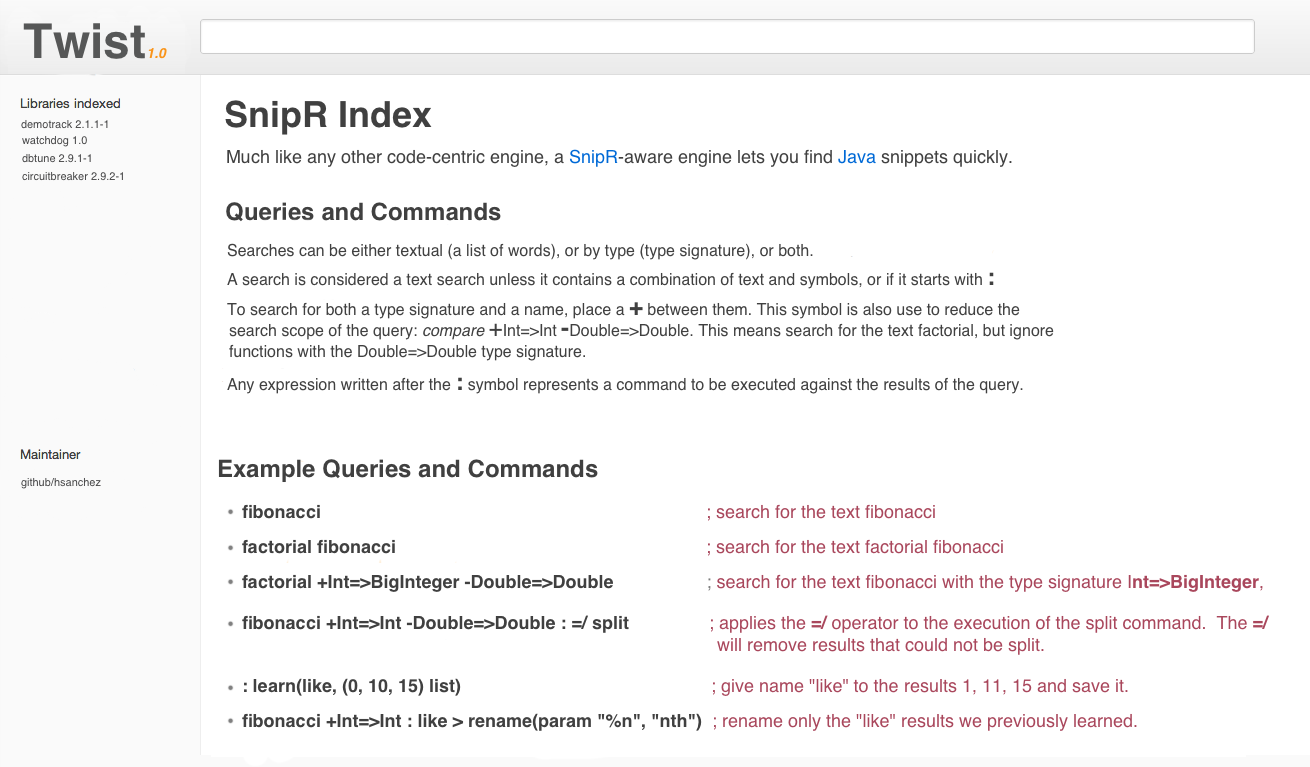
\includegraphics[width=\textwidth]{images/twistsite}
    \caption{Twist's Web Interface.}
    \label{fig:twist}
\end{figure}
% \pagebreak

To start gathering code examples, Olivia issues a query targeting Facebook APIs written in Java. Olivia specifically looks for functionality that deals with status or post updates. She does not want any Android\footnote{\url{http://www.android.com}} specific source code. Consequently, Olivia's first query will contain a list of words matching her intent and a reduction in search scope. Figure~\ref{fig:twistquery} shows this query and the results produced by it. 

\begin{figure}[!ht]
    \centering
    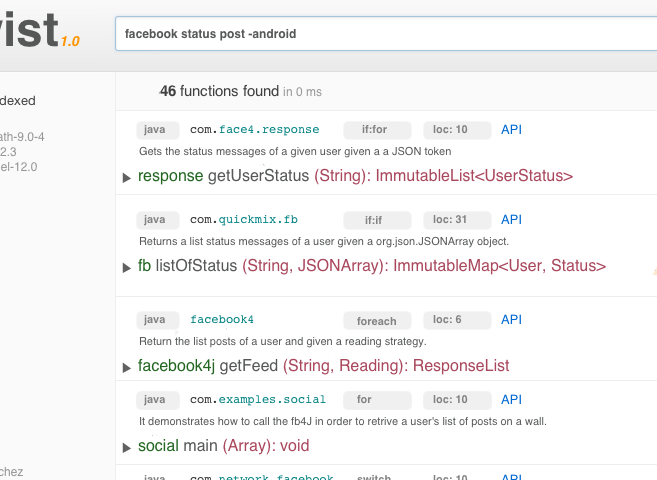
\includegraphics[width=\textwidth]{images/twistquery}
    \caption{Olvia's first query, which targets Facebook APIs written in Java.}
    \label{fig:twistquery}
\end{figure}
% \pagebreak

She tries to screen all of the results but gives up after some time. She does not have time to look at every single result. Consequently, she will use Twist's functionality to her own advantage. She issues a command that will reject those results which size exceeds 20 lines of code (Figure~\ref{fig:twistslash}). The output of this command is clearly more manageable for Olivia. Consequently, Olivia's screening efforts will be reduced.

\begin{figure}[!ht]
    \centering
    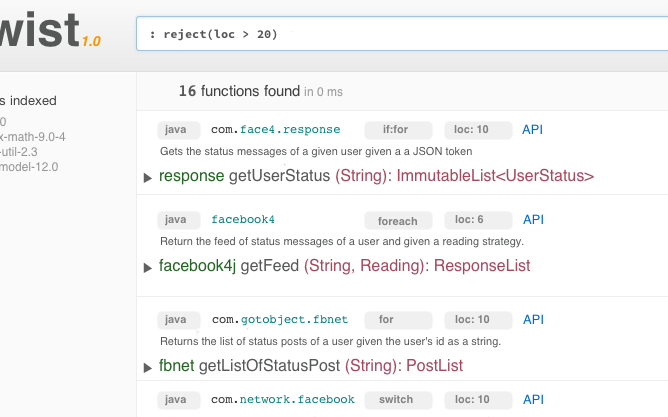
\includegraphics[width=\textwidth]{images/twistslash}
    \caption{Olivia rejects the code examples whose size exceeds 20 lines of code. The 
	 reject operation takes as an input the list of current results and an anonymous function, 
	 which is applied to every result in that list.}
    \label{fig:twistslash}
\end{figure}  

Some of these results (Figure~\ref{fig:twistslash}) have highly coupled dependencies that Olivia is not interested in using, such as ImmutableList from the Google's Guava library\footnote{\url{http://code.google.com/p/guava-libraries/}}. She then issues a retargeting request that will replace those dependencies with APIs found in the Java SDK. Olivia can specify these dependencies by typing an associated abbreviation; e.g., ImmutableList can be written as IL or ImL. The execution of this request reloads the Twist page, listing the successfully retargeted snippets and adding red markers next to the failed-to-retarget snippets.  These markers can point Olivia at which results she should not spend any retargeting effort from now on. Figure~\ref{fig:twistretarget} shows this command and the results produced by it\footnote{favorites is a sub list extracted from list and its defined as: learn(favorites, (0, 1, ...) list )}. 

\begin{figure}[!ht]
    \centering
    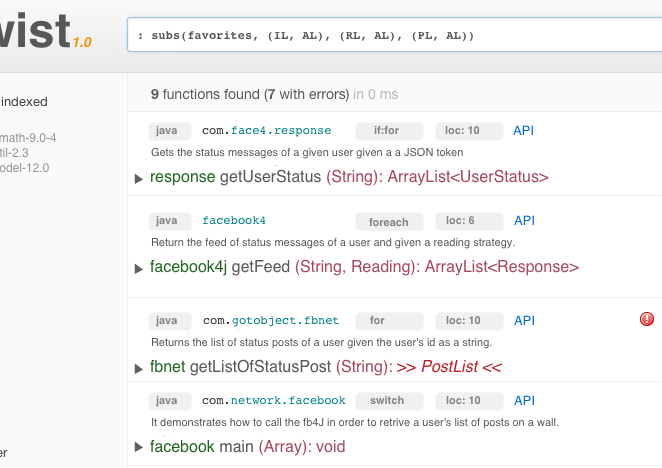
\includegraphics[width=\textwidth]{images/twistretarget}
    \caption{Olivia issues the subs command, which will replace one type for 
	 another.}
    \label{fig:twistretarget}
\end{figure} 

For Olivia, the whole idea of having the failed-to-retarget snippets around is distracting. Therefore, she issues another command which will drop any failed-to-retarget results from the current list of results. Figure~\ref{fig:twistclean} shows this action. 

\begin{figure}[!ht]
    \centering
    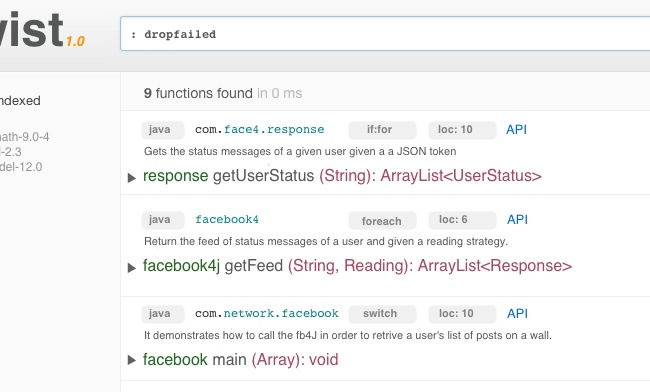
\includegraphics[width=\textwidth]{images/twistclean}
    \caption{Olivia issues a user-defined command, named dropfailed, which will drop 
	 any failed-to-retarget results from the current list. The dropfailed was defined as : 
	 learn(dropfailed, reject(list, err == false))}
    \label{fig:twistclean}
\end{figure}   

She arbitrarily clicks on individual results---a result found in the result set---that she sees as promising for additional retargeting. This action offers the choice for further retargeting to gain more confidence of these results' suitability (see Figure~\ref{fig:basealternative} for an example). She then invokes a few additional commands: rename functions, and change a condition-controlled loop (e.g., for loop) to another one (e.g., while loop), matching what Olivia had in mind for how and what status updates are obtained\footnote{This process can continue (See Eager retargeting policy in Section~\ref{sec:eagervslazy}) until Olivia decides to stop.}. Again, those unsuitable results will be filtered out and thus reducing the number of results to be inspected by Olivia.

Continuing her information gathering, Olivia may continue retargeting results until there are no more results to screen or to not like any of the different variations. This can happen, which can lead Olivia to modify her previous queries to obtain similar or different results than she had previously obtained.

When she is satisfied with the resulting code example, she can evaluate these results in more detail and thus pick the most suitable example she can integrate into her own code.


\chapter{Algorithms}{}
\label{chap:algorithms}

\lettrine[lraise=0.1, nindent=0em, slope=-.5em]{N}{OW THAT THE POLICY} behind \uppercase{SNIPR} has been stated, the next step is to describe the problem the SNIPR's algorithms plan to solve.
% 
% In most programming settings, manually performing program transformations on a large collection of snippets is error prone and cumbersome, while programming solutions from scratch is often beyond the skill-set of most programmers. Consequently, it is more practical to use program transformation systems to take some of the burden of manually performing transformations off the developers.

Most code search approaches that use program transformations start with specifying automated program transformation procedures and parameterizing source code text fragments, and derive either: (1) hierarchical code generation rules~\cite{Nita:2010en} for runtime-code generation, (2) new or alternative program implementations~\cite{Wightman:2012gc}, or (3) domain specific languages for program adaptation~\cite{Visser:2001tc}.

While these outcomes have indeed proven successful, they still impose a significant manual effort on the developers---e.g., developers need to spend additional effort to make these solutions configurable and ready to go. Consequently, these methods are impractical if they are to be used---as is---in a \uppercase{SNIPR}-aware code search engine. 

The above observation is the motivation for the algorithms discussed in this chapter. The aim of these algorithms is to efficiently learn and use coherent mapping-based program transformations. By applying these transformations to a snippet, \uppercase{SnipR} can convert the structure of one snippet into the structure of another. The goal is for this to happen with minimal or no cost to the developer.

Briefly, these algorithms represent the modules required to implement \uppercase{SnipR} functionality. These modules are illustrated in Figure~\ref{fig:sniprentire}. The Setup and Learning steps occur at indexing time. Given a set of indexed snippets, the Setup step populates the \emph{Snippet Space} by invoking a code clone searching and detection tool and then considering all the possible combinations of (original-clone) pairs. The output of the Setup step is fed into the Learning step. The Learning step then builds mappings for all the (original-clone) pairs in the \emph{Snippet Space}. When invoking \uppercase{SnipR}, Twist interprets this input by searching a mapping that will make sense of this input (See Chapter~\ref{chap:twist} for details). At this point, the Matching step maps the retargeting request to its corresponding optimal mapping and then applies this optimal mapping to the original snippet.

\begin{figure}[!ht]
    \centering
    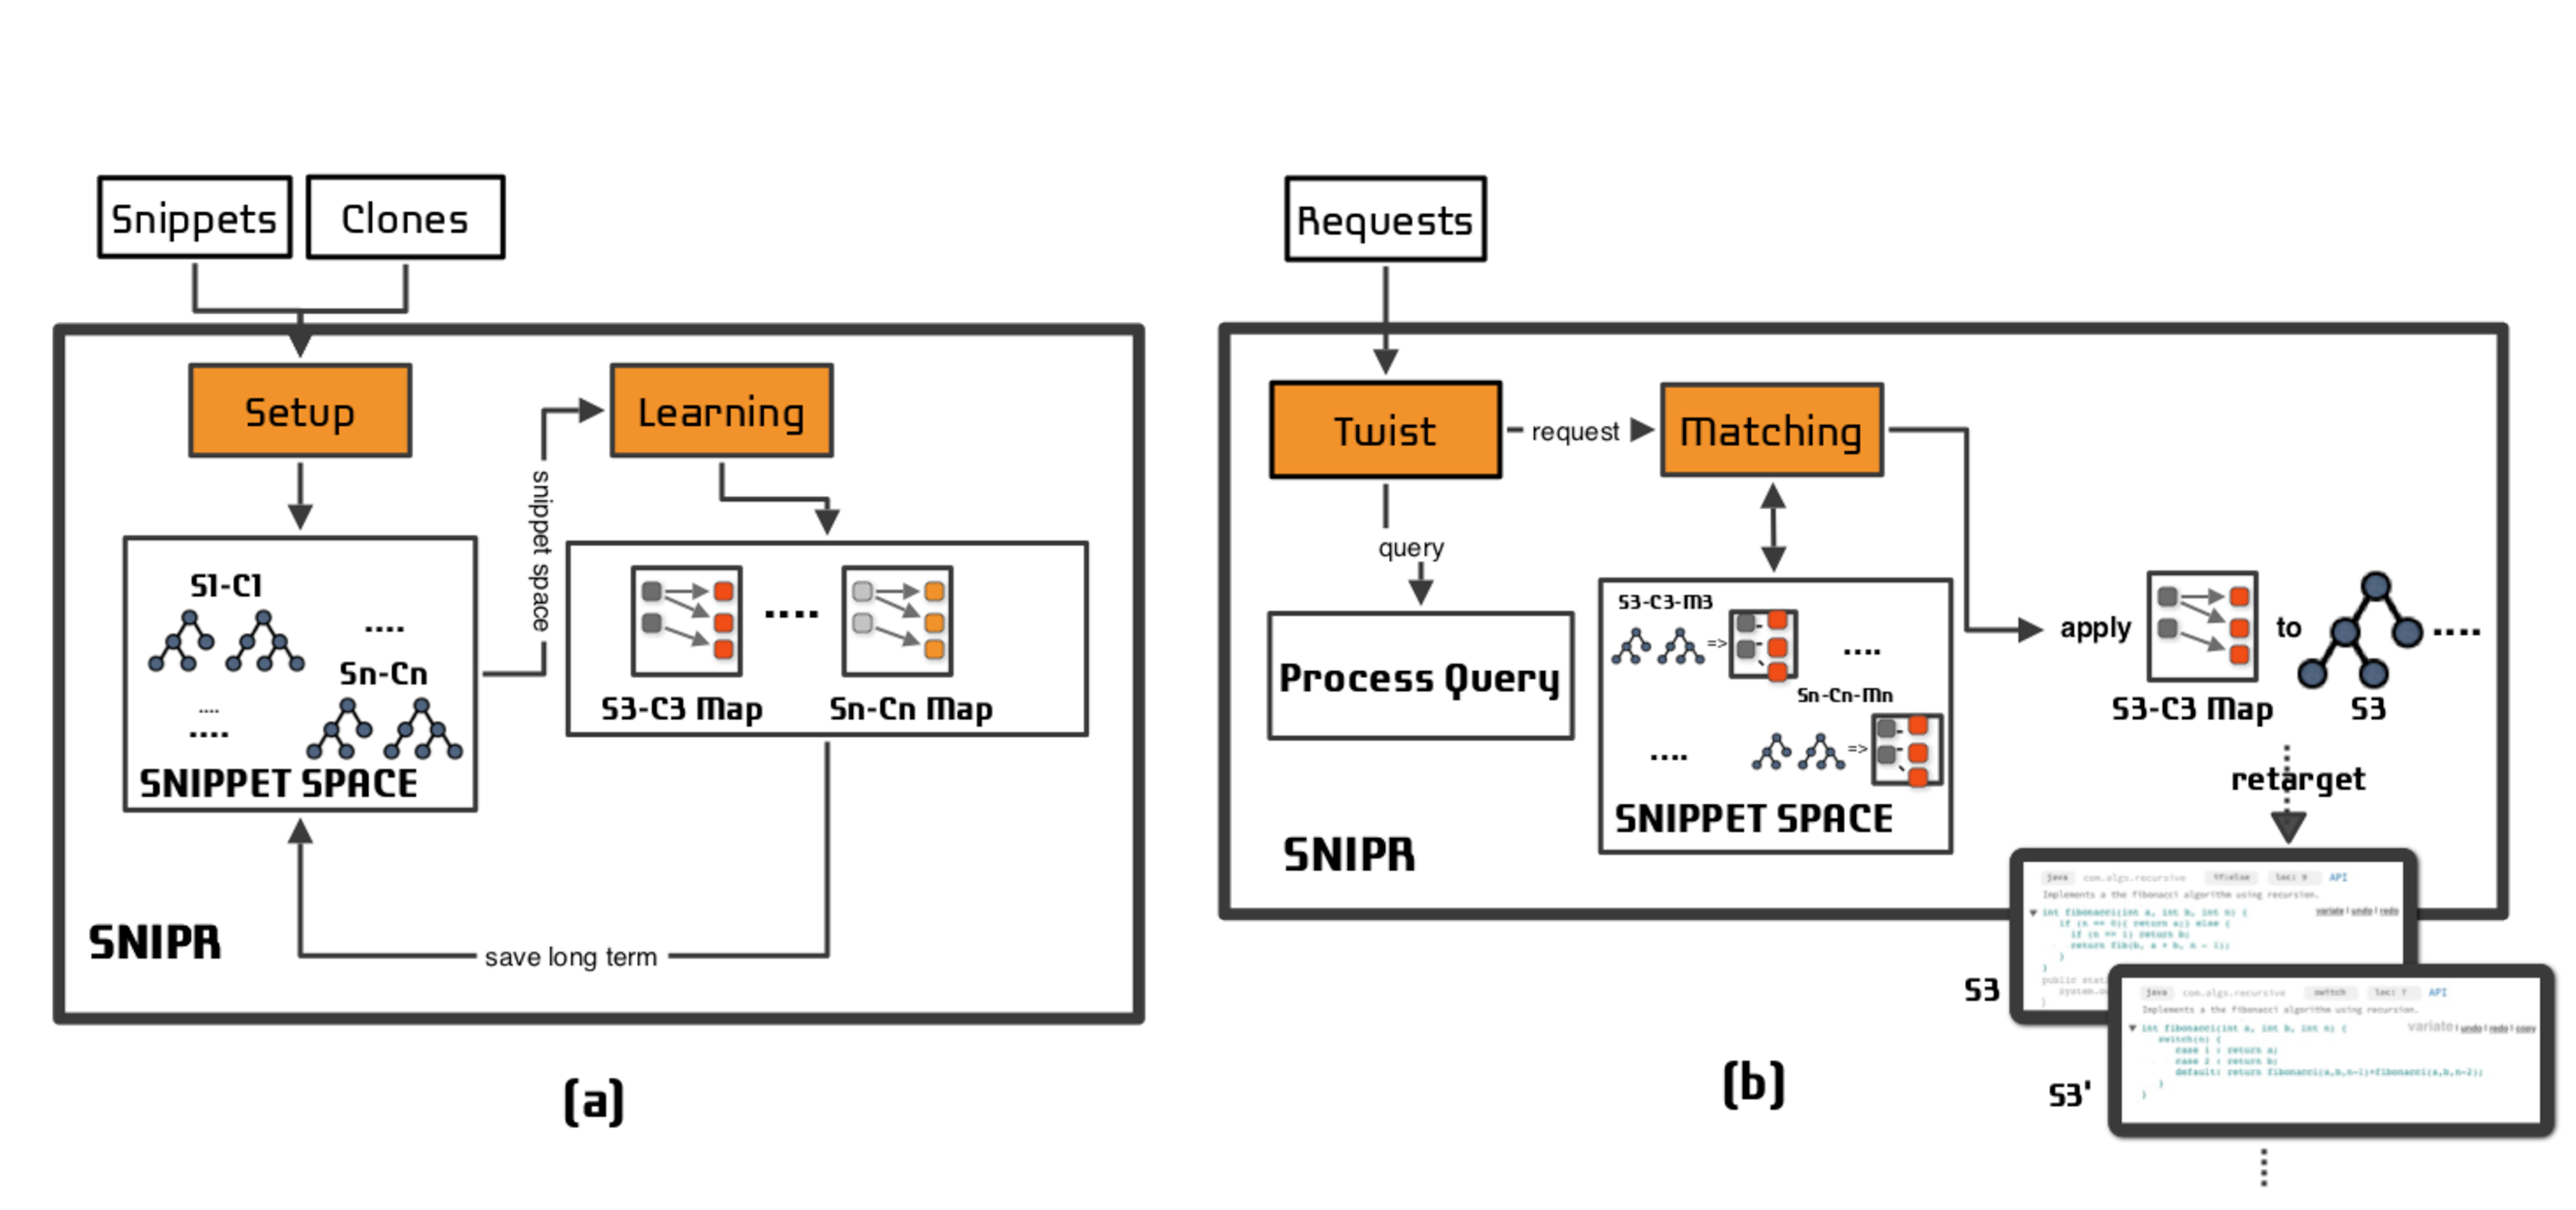
\includegraphics[width=\textwidth]{images/SnippetRetargetingApproach}
    \caption{SNIPR's Overall Architecture: Figure (a) shows how SNIPR is setup. Figure (b) shows SNIPR in action.}
    \label{fig:sniprentire}
\end{figure}

In the reminder of this chapter, the algorithms or steps \uppercase{SnipR} needs to set-up and do code retargeting in a snippet-centric search engine are described in more detail. 

\fancybreak{\pfbreakdisplay}

\section{The Setup Step}
\label{sec:precomputation}

This algorithm relies on state-of-art approaches in code clone searching and detection~\cite{Jiang:2007cj, Roh:2010ts} in order to reveal, per an indexed snippet, a set of snippet alternatives (clones). These clones are needed to realize how \uppercase{SnipR}'s learning algorithm operates. By definition, clones are related implementations and thus similar. They are also syntactically different and are indeed \emph{interchangeable}. This knowledge is used by the learning algorithm to hypothesize and map together related code elements between snippets. 

This algorithm is based on the following intuition. Even though code clone searching and detection tools, called CSD from now on, might consider a tremendous space of alternative snippets for a single snippet, the number of unique snippet alternatives and therefore the number of snippet instances to use is much lower. Consequently, it makes sense to cache and reuse the set of unique alternative snippets computed by CSD, instead of performing multiple invocations only to compute the same snippets multiple times. The resulting set of (original-clone) pairs---$S = \{(s_1, s_2) x (s_1, s_3) x (s_1, s_4) ... x (s_1, s_n)\}$---will be saved in the \emph{Snippet Space} (cached snippets). This space, or the output of this algorithm, is computed by considering all the possible combinations of (original-clone) pairs that can be revealed by using an original snippet and its clones. The \emph{Snippet Space} is maintained in the same way indexes are maintained in a search engine.

For a larger number of libraries, the setup of a \emph{Snippet Space} becomes expensive, as a larger number of calls to CSD are required. To reduce this burden, the setup step builds the \emph{Snippet Space} incrementally, in-sync with the most popular libraries searched by users. By doing this, there is no need to consider all the possible combinations of (original-clone) pairs upfront; only a subset will be suffice.

\fancybreak{\pfbreakdisplay}

\section{The Learning Step}
\label{sec:learning}

This section discusses, at a very high level, the learning algorithm for building mapping-based program transformations. These programming transformations allow \uppercase{SnipR} to transfer structure between similar code snippets; i.e., perform code retargeting. 

To learn code mappings in a principled way, we leverage techniques in structured prediction~\cite{Collins:2002uo}, which involve predicting objects with complex internal structure and dependencies---e.g., parse trees~\cite{Kumar:2011uj}. In particular, we cast the problem as a translation discovery problem: given a source and a clone snippet respectively, we induce a translation table over their similar structures. This table specifies how two code snippets correspond. Once induced, this table can be used to determine structure translation candidates and thus synthesize a code mapping between two snippets. 

The core of this algorithm is based on the hypothesis that a general code retargeting scheme can be produced by training a machine learning algorithm (machine learner) based on human-generated mappings (human-generated corpus). The machine learner can use the knowledge gained from the collected corpus to learn how to build mappings from further snippets using only what it learned during training. The entries of these mappings will specify how two related snippets correspond to one another (Figure~\ref{fig:mappings}). SNIPR uses these mappings to automate the process of changing the structure of one snippet to the structure of another. Mappings of this kind have an abstract syntax similar to the mapping syntax proposed by Nita and Notkin in their paper~\cite{Nita:2010en}.

\begin{figure}[!ht]
    \centering
    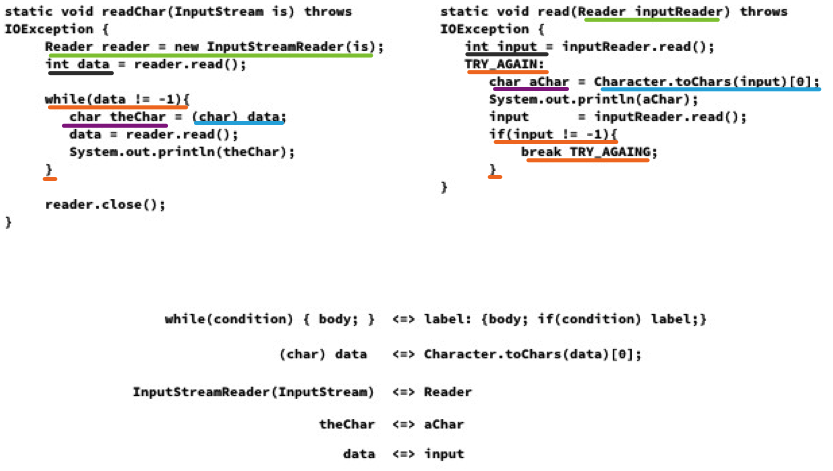
\includegraphics[width=\textwidth]{images/mappings}
    \caption{A simple mapping between two snippets.}
    \label{fig:mappings}
\end{figure}

Based on the above observation, the learning algorithm will use structured prediction---e.g., the generalized Perceptron~\cite{Collins:2002uo}---to learn how to write these code mappings. The corpus of human-generated mappings will be collected via a Web-based crowdsourcing application; the plan is to use either the Amazon's MechanicalTurk or a very basic Web application where users explicitly transform one snippet into another and map related code elements together. This information is used to train the machine learner.

In a nutshell, the learning algorithm takes as an input the \emph{Snippet Space}---computed by the setup step (See Section~\ref{sec:precomputation})---and a set of user constraints, such as data accessibility or function arity. These user constraints will help determine feasible regions, which are code areas where code retargeting can be applied. These user constraints will be empirically determined. This algorithm will use syntactic analysis, in conjunction with these constraints, to help determine these areas. The feasibility of these areas is affected by different factors, such as the extent of local data declaration, control scope within functions, etc. Figure~\ref{fig:mappinggeneration} shows this process applied to a pair of snippets:

\begin{figure}[!ht]
    \centering
    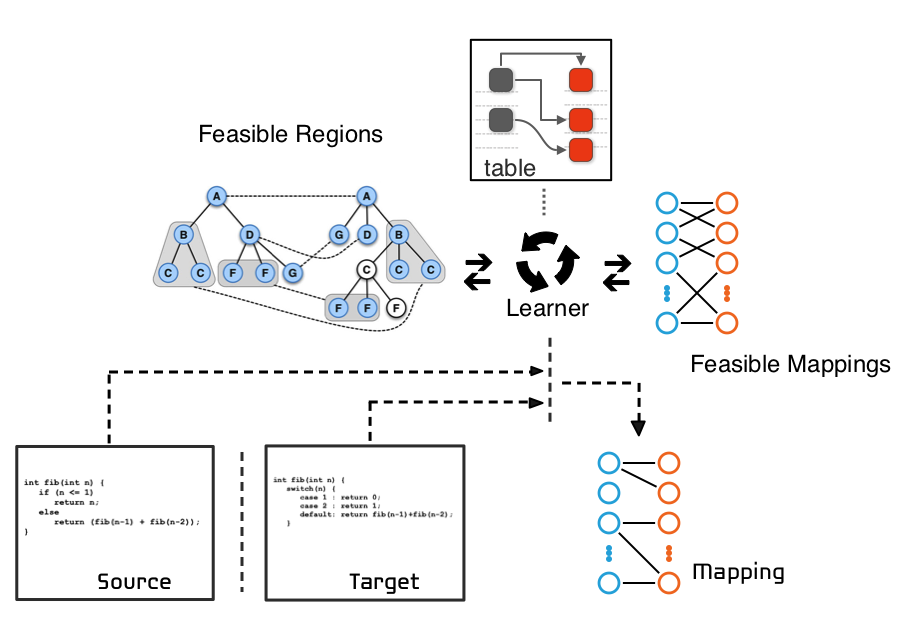
\includegraphics[width=\textwidth]{images/mappinggeneration}
    \caption{Learning a mapping-based transformation.}
    \label{fig:mappinggeneration}
\end{figure}

\fancybreak{\pfbreakdisplay}

\section{The Matching Step}
\label{sec:matching}

This algorithm is responsible for determining the optimal mapping for a given retargeting request and applying it to a snippet implementation. \uppercase{SNIPR} will use a set of heuristics, in the form of a matching logic, that given a retargeting request, will efficiently assign the corresponding optimal mapping for each result. 

At a very high level, this algorithm takes as an input a query and a retargeting request (See Chapter~\ref{chap:twist}). Given this information, the matching step takes every mapping that explains the input. A variation of the explanatory power scheme, suggested in~\cite{Little:2008hr}, determines how well every mapping explains a sequence of tokens obtained from the input. This scheme states that tokens can be explained in numerous ways. One example could be a token that is matched with a function name is explained as invoking that function, and a token that is matched as part of a string is explained as helping create that string. Once the input is mapped to its corresponding optimal code mapping, the algorithm applies this code mapping to the original snippet implementation. This action produces a variation containing the changes specified by the mapping. Otherwise, it reports any found errors to the developer. 

This chapter has introduced the algorithms SNIPR uses to learn and use mapping-based program transformations in a code-centric search engine. To recap, these algorithms are the Setup Step, the Learning Step, and the Matching Step.

\chapter{Twist}{}
\label{chap:twist}

\lettrine[lraise=0.1, nindent=0em, slope=-.5em]{T}{HIS CHAPTER INTRODUCES} Twist, a language for interacting with search results, and combining and executing code retargeting operations. 

\section{Twist}
\label{sec:twist}

Twist is an experiment in designing a simple language for combining, and executing code retargeting operations---directly from the search box---with a syntax inspired by multiple languages, such as C, and Io. This chapter will go over its focus, philosophy, core syntax, built-in functions, and how to run it.

\subsection{Twist's Focus}
\label{sec:focus}

Typically, most code examples come from libraries, which are often made of a set of static and instance methods defined within a Java class. Most of these libraries address a specific computational task by either creating or combining these methods. This form of modular programming has important benefits~\cite{Sedgewick:2011tx}. Some of these benefits include 

\begin{enumerate}
	\item One could deal with modules of reasonable size.
	\item One could share and reuse code without having to reimplement it.
	\item One could substitute improved implementations.
	\item One could develop abstract models for addressing programming problems.
\end{enumerate}

These benefits are applicable to search-driven programming. Consequently, the preliminary design of code retargeting operations will be heavily influenced by the type of changes that could be made to modules (methods that properly implement an API).

\subsection{Twist's Philosophy}
\label{sec:philosophy}

The goal of Twist is to explore the unification of text searches and code retargeting, so the trade offs tend to favor simplicity and flexibility, over performance. While performance(in terms of computational throughput) is highly important, it is not a top priority. The code retargeting functionality will be designed to be as intuitive and concise as possible, and tailor performance around the design of the language. Figure~\ref{fig:focalpoints} shows the relative emphasis between three design goals.

\begin{figure}[!ht]
    \centering
    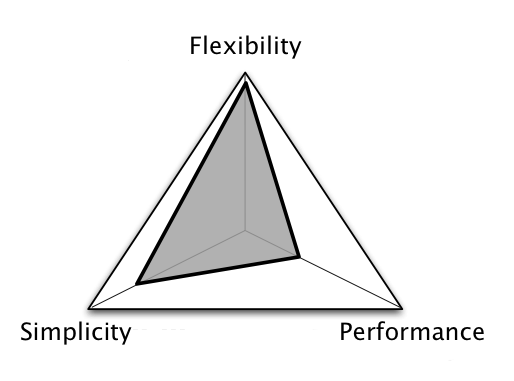
\includegraphics[width=\textwidth]{images/focalpoints}
    \caption{Relative emphasis between three design goals.}
    \label{fig:focalpoints}
\end{figure}

\subsection{Twist's Core Syntax}
\label{sec:syntax}

Twist has a very simple syntax. It has three expression types: 

\begin{enumerate}
	\item Atoms: names, identifiers, and other literals.
	\item Lists: an ordered set of other expressions. 
	\item Calls: a pair of expressions.
\end{enumerate}

This means that every expression in Twist, derived from these three expression types, can be \emph{desugared} to these core elements. The rest of the sections below describes the rest of the syntax.

\subsubsection{Names}
\label{sec:names}

Names are one of the simplest syntactical elements in Twist. They are used for prefix function calls and don't trigger any special parsing. They start with a letter, and don't contain any colons. For example, 

\begin{minted}{java}
what?!, What?!, and WhAt?! 
\end{minted} 

are all the same.

\subsubsection{Operators}
\label{sec:operators}

Operators are a special case in the Twist's syntax. They are parsed like in Io. The Twist's parser intercepts any operator defined by the interpreter, and translate them to method calls. The fact that they do not require explicit parenthesis is convenient. For example, the expression

\begin{minted}{java}
: 1 + 10 * 9 + 1
\end{minted}

is equivalent to

\begin{minted}{java}
: 1 + (10 * (9)) + (1)
\end{minted}

Operators in Twist have a little  bit of operator precedence. Twist has the same operator precedence as with the C language precedence levels.

In addition to these operators, Twist supports three special operators: the braces (\{;\}) operator, the chain (>) operator, and the slash (/>) operator.

The \{;\} is a left-to-right operator. This operator helps express a series of operations that are executed in order. This series of operations, separated by semicolons and surrounded by curly braces, is a syntactical sugar for a ``do'' method call. So this

\begin{minted}{java}
: {display("Hello, World!"); display(1 + 2)}
\end{minted}

is equivalent to

\begin{minted}{java}
: do(display("Hello, World!"); display(1 + 2))
\end{minted}

The > is also a left-to-right operator. This operator helps express nested operations and data flow.  The > operator forms a syntactic glue that binds operations together. For example, the user might think of values passing through a sequence of code transformations---from left to right.

\begin{minted}{java}
: rename-param (
	twitter, facebook) > 
	split > subs ((TS, FS))
\end{minted}

is equivalent to:

\begin{minted}{java}
: subs(split(rename-param(twitter, 
	 facebook)), (TS, FS))
\end{minted}

where:

\begin{enumerate}
	% \item \_ is a placeholder for the output of a previous method call.
	\item The rename command returns the list of results where the parameter ``twitter'' was 
	renamed.
	\item The split command returns the list of functions produced by the split command.
	\item The subs command replaces the TwitterService (abbreviated as TS) type for the 
	FacebookService (FS) type.
\end{enumerate}

The /> operator is similar to the > operator. It differs from the > in the sense of it will attempt to cut down on any failed results, which are a product of the execution of Twist's operations. The following example demonstrates this command. The statement before the : separator is a query. Like this:

\begin{minted}{java}
: factorial +Double => Double : subs(
	(Double, Int)
	 ) /> rename-param(n, nth) 
\end{minted}

Any results, after the application of Twist's /> operator, containing any syntactic or parsing errors will be filtered out from the produced results. Semantic errors will be outside the scope of Twist's functionality. By omitting this operator, developers are willing to see these failed results in the results list.

\subsubsection{Lists}
\label{sec:lists}

A list can be created by separating functions with commas. For example:

\begin{minted}{java}
: 1, 2, 3
\end{minted}

Parentheses are not necessary, but they are often useful since commas have low precedence. For example:

\begin{minted}{java}
: hello a, b     ; means (hello(a), b)
\end{minted}

is different than

\begin{minted}{java}
: hello(a, b)    ; means hello(a, b)
\end{minted}

\subsubsection{Functions}
\label{sec:functions}

In Twist, a name followed by an expression will call that named function and pass it the given argument(s)---if provided. For example:

\begin{minted}{java}
: version (1.0, true)
\end{minted}

This is a function with two arguments. If the version function had zero arguments, then it would look like this:

\begin{minted}{java}
: version
\end{minted}

This function with zero arguments prints the current version of Twist. With two arguments, it prints additional information in regards to Twist's 1.0 version, such as changes that went in version 1.0. 

That's the basic syntax. The Twist parser reads that and then it translates it to the core syntax.

\section{Running Twist}
\label{sec:running}

Twist is also a Web application, and one can access it by using a Web browser. Once opened, the Twist's REPL will start. The command line interface for this interpreter is showed in the Figure~\ref{fig:twist}. 

\subsection{Twist's Interpreter}
\label{sec:interpreter}

A good way to learn Twist is to interact with an interpreter and study its responses. This is very similar to the way people already interact with search engines. For this work, two types of interaction with Twist are considered: 

\begin{enumerate}
	\item Supply an expression, sometimes led by a text search, to be evaluated.
	\item Import a script file with a set of expressions to be evaluated. 
\end{enumerate}	

The following image (Figure~\ref{fig:runtime}) represent the processing of commands issued by a user and handled by Twist:

\begin{figure}[!ht]
    \centering
    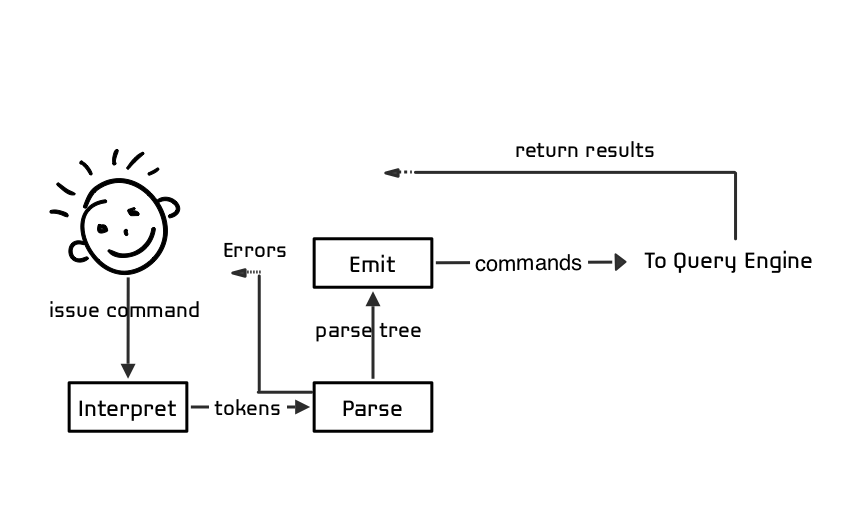
\includegraphics[width=\textwidth]{images/runtime}
    \caption{Twist's runtime processing.}
    \label{fig:runtime}
\end{figure} 

Any errors caused by misusing Twist's syntax and built-in functionality will be displayed to the user right after the user has pressed the enter key. Figure~\ref{fig:error} displays this.

\begin{figure}[!ht]
    \centering
    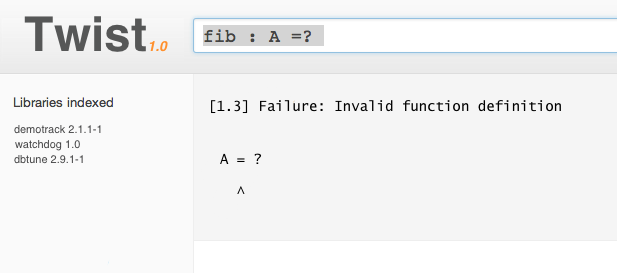
\includegraphics[width=\textwidth]{images/error}
    \caption{Error caused my misusing Twist's syntax and built-in operations.}
    \label{fig:error}
\end{figure}

\subsection{Built-in Functions}
\label{sec:functions}
 
As of now, only a few built-in functions have been designed:

\begin{enumerate}
	\item do <expr>: If the <expr> is anything but a list, Twist will evaluate it and 
	return. If it is a list, then Twist will evaluate each item in the list, in order, 
	and then return the evaluated value.
	
	\item <params> = <body>: It creates an anonymous function. <params> should either be 
	a single name or a list of parameter names. <body> represents the body of a 
	function. It is also an expression. For example, : (a = loc(a) < 20) is an 
	anonymous function that returns true if a snippet's size is less than 20 lines of 
	code. 
	
	\item if(<predicate>, then-clause, else-clause): Twist evaluates the predicate. If 
	the predicate evaluates to true, then it evaluates and returns the <expr>. Otherwise, 
	it will evaluate and return the <expr> in the else clause. For example, : if(true 
	\&\& true, display ``Y'', display ``N'').
	
	\item learn(<name>, <expr>): Twist binds a value to a variable in the current scope. 
	<name> should be a single name. Twist will evaluate <expr> and then it will bound the 
	result to the name. For example, : learn(twist, ``SNIPR's tiny language'' )
   
	\item isbool? <expr>, isint? <expr>, islist? <expr>, isname? <expr>, isunit? <expr>: Twist 
	evaluates <expr>, and then returns true if the result is the given type.
 	
	\item <int> <expr>: Twist evaluates <expr>, expecting to be a list. Then, it will 
	return the item at the <int> position in the list. For example, : 2 (1, 2, 3) will 
	return 3.
	
	\item size <expr>: Twist evaluates <expr>, expecting it to be a list. Then, it will 
	return the size of the list.
\end{enumerate}

\subsection{Built-in Commands}
\label{sec:retargetingops}

Only a few built-in commands are designed:

\begin{enumerate}
	\item import <url>: The command will import a twist file containing a set of 
	user-defined functions. Once the twist file is loaded, any function in the file will 
	be interpreted by the Twist's interpreter and ready to be used by the user.
	
	\item list: It returns the current list of results, or () if it is empty.
	
	\item select(<list>, <predicate>): It applies the <predicate>(usually an anonymous function) 
	to the given list of results. When using the current list of results (results produced by a 
	query) or using the > or /> operators, the list is implicit in the operation. Therefore it can 
	be omitted. For example, fibonacci +Int=>Int : select(loc > 20), which is the same as 
	fibonacci +Int=>Int : select(list, a = loc(a) > 20). Or, fibonacci +Int=>Int : select(loc > 
	20) > select(loc < 7).
	
	\item apply(<list>, <operation>): It applies an <operation>(e.g., a retargeting operation) 
	to the given list of results. Similar to the select operation, the list of results can be 
	omitted. For example, fibonacci +Int=>Int : apply(rename-method(from, to)). Or, fibonacci 
	+Int=>Int : apply(rename-method\footnote{learn(rename-method, a, b, name(method(a), b))}(from, 
	to)) > apply(rename-param\footnote{learn(rename-param, a, b, name(param(a), b))}(from, to)).
		
	\item reject(<list>, <predicate>): It is similar to the select operation. The main difference 
	is that instead of selecting those results that matched the predicate, it will reject those 
	ones who do. 
	
	\item undo, redo: The undo command rolls back a change made to one or more results. 
	The redo is the opposite to the undo command.  
	
	\item loc(<result>): It returns the size of snippet (represented as a result in the 
	list of results produced by a query). When using this operation within the select and reject 
	operations, the <result> is implicit in the operation; therefore it can be omitted. 
	
	\item morph(<list>, <pairs-of-statements>): It tries to change from one type of statement 
	(e.g., switch statement) to another type (e.g., a series of if:else statements). Returning an 
	error if the change cannot be made. Similar to the select, apply, and reject operations, the 
	list of results can be omitted (this is the same for the rest of operations). For example, : 
	morph((if:else, switch)) (Figure~\ref{fig:basealternative} shows such a transformation).  
	
	\item err(result): It returns true if the result contains syntactic (parsing) errors. 
	It returns false otherwise. Similar to the loc operation, when used in the select and reject 
	operations, the <result> can be omitted.
	
	\item subs(<list>, <pairs-of-types>). It replaces one type for another. The 
	<pairs-of-types> is a list of source-target pairs. For example, : subs((Int, Double),
	(ArrayList, LinkedList)).
	
	\item split(<list>, <int> = 2): It splits a method into <int> parts. Returning an 
	error if the change cannot be made. If <int> is not specified, the it is assumed that the user 
	wants to split the method into two methods. For example, fibonacci +Int=>Int : split

   \item merge(<list>, <list-of-methods>, <method>): This is the opposite of the split command. 
	For example, fibonacci +Int=>Int : merge((method(fib\_helper), method(fib)))
	
	\item param <name>, method <name>: It returns either a param matching a given name, 
	or a method matching a given name.
	
	\item name (<member>, <new-name>): It gives a new name to an existing member (parameter in 
	a method, or the name of the method).
	
\end{enumerate}

\subsection{Mixing Queries and Commands}
\label{sec:queriescommands}

Code searches can be either textual (a list of words), or by type (type signature\footnote{<InputTypes>=><OutputType>}), or both. A search is considered a text search unless it contains a combination of text and symbols, or if starts with `:'. To search for both a type signature and a name, place the + symbol between them. Any expression written after the : symbol represents a command to be executed against the results of a query. A few examples are illustrated below:

\begin{minted}{java}
// search for the text fibonacci	
fibonacci
// search for text factorial and the 
// text fibonacci
factorial fibonacci
// search for the text fibonacci, with 
// the type signature Int=>BigInteger 
fibonacci +Int=>BigInteger 
// gives a name to the first item in the 
// current list of results.
: learn(first, 0 (list))
// rename the first item's parameter 
// from n to number.
fibonacci +Int=>Int : first > 
rename-param(n, number) 
\end{minted}
	 
Let's make one important observation. The + symbol, besides helping search by type, can be used to reduce the search scope of a query. For example, if one knows in advance what library (separated by comma if there are more than one library) to search, then one can use the + (it means ``only in'') to specify the name of the library. Like this:

\begin{minted}{java}
: fibonacci +supermath-1.0 
\end{minted}

The opposite of + symbol is the - symbol. This symbol means ``everywhere except in.'' The following example illustrates this behavior.

\begin{minted}{java}
: fibonacci +like-1.0 -dontlike-1.0
\end{minted}
 
 
This chapter has introduced Twist, a language for interacting with search results, and combining and executing code retargeting operations. 

\chapter{Proposed Solutions}{}
\label{sec:solutions}

\section{Designing \uppercase{SnipR} operations that could be invoked directly from the search box (RQ1)}
\label{sec:rq1}
Unpacking this a bit, the key idea is to design a set of retargeting operations or commands that could be invoked from the search box, without losing any sight of the current search goal (See Chapter~\ref{chap:twist} for more details). This design should balance two inter-related principles: simplicity and flexibility. To understand what's needed to produce this type of design, this research will turn to the seminal work on sloppy command lines for the Web~\cite{Little:2007dh, Miller:2008ge} and on platform-specific linguistic command lines~\cite{Raskin:2008wb}. Similar to both types of work, the \uppercase{SnipR}'s command line will have flexible syntax requirements. This flexibility offers an important advantage. It allows queries and retargeting requests to be intermixed---or used separately. The focus of these commands---and language---will be twofold. First, to interact with search result. Second, to perform code modifications on retrieved code examples. For simplicity, SNIPR will provide most of the mechanisms for expression and control of changes that could be made to modules (methods that implement an API). This involves discovering the fundamental concepts of retargeting modules, to extract them from their various reincarnations, and to present them in a pure and distilled form. This form will be inspired by the syntax of the Io programming language\footnote{\url{http://iolanguage.org/}}. For flexibility, a simple language for combining, and executing code retargeting commands will be developed. This language's goal is to extend \uppercase{SnipR}'s available functionality. 
% Previous work in command lines for code modifications exist and could be usually seen implemented as plugins in mainstream IDEs, such as Eclipse\footnote{\url{http://www.eclipse.org}} and IntelliJ IDEA\footnote{\url{http://www.jetbrains.com}}. In contrast, with \uppercase{SnipR}, developers will continue to use their Web browser to do these code modifications. 

\fancybreak{\pfbreakdisplay}

\section{Performing Code Retargeting (RQ2, RQ3, and RQ4)}
\label{sec:restqs}
Code modification---to make code more suited---or retargeting is an operation that can work on a single search result or an entire result set. Therefore, this operation requires that those cases where code mappings can be learned and/or applied are carefully identified. This will prevent any unnecessary work from happening as matched code examples are being returned by the query engine. This requirement will be addressed by developing a set of reliable and cache conscious \uppercase{SnipR} algorithms (RQ2). They should be reliable in the sense of consistently learning code mappings from example code. They should be cache conscious in the sense of exploiting recently read example code if this code must be read again in the future. The output of these algorithms are code mappings that are applied by the query engine when retargeting is needed (See Chapter~\ref{chap:algorithms} for more details). In order for the query engine to do that, a set of code retargeting operators well-suited for manipulating example code within query processing must be created (RQ2). These operators should be reliable in the sense of applying learned mappings. Moreover, they should be implemented within the querying processing step of a working code search engine (RQ3). 

As for the rules that would guide the retargeting of found code, this research will turn to developing a prototype, which will represent code searching as a short cycle of alternating query, retarget (or the intermixing thereof), and screen phases. By leveraging the experience gained with this prototype, a model for retargeting found code will be developed. This model will allow a formal reasoning about any experimentation in the \uppercase{SnipR}'s design space, and a path to an efficient implementation of \uppercase{SnipR}. 

In retrospect, if the developer retargets code in advance, then the evaluation results are available immediately, which saves valuable time searching for appropriate example code (See Figure~\ref{fig:retargeting}). By saving this time, the developers will get the work done more quickly (RQ4). This will be possible only if \uppercase{SnipR}'s retargeting operations are efficient, which will be demonstrated by answering RQ2. 

% Previous work in adapting code to alternate contexts and/or to new APIs exist. Such work has helped developers with many development tasks, such as adapting example code to new contexts~\cite{Wightman:2012gc} or to new APIs~\cite{Nita:2010en}. This also includes resolving many simple coding errors quickly\footnote{{Quick Fix Scout: \url{https://code.google.com/p/quick-fix-scout/}}, {EUKLAS: \url{http://www.cs.cmu.edu/~euklas}}}, or suggesting ways for correcting compiler and runtime errors~\cite{Hartmann:2010hx}. Unlike \uppercase{SnipR}, any interaction for finding and changing any example code or suggesting solutions to a problem in the developer's code is directly done in the IDE.

\fancybreak{\pfbreakdisplay}

\section{Evaluation}
\label{sec:evaluate}

The evaluation methodology to be followed is to validate the \uppercase{SnipR} approach and results through user and lab studies. The tests will be run on \uppercase{SnipR} prototypes in a working code search system, such as Sourcerer\cite{Bajracharya:2006vn} or another Internet-scale code search engine. The user studies will involve a list of subjects, solicited from a public mailing list at a college campus. The subjects will also be experienced Web users, have some programming experience, and could type reasonably well. The use and test of the \uppercase{SnipR} prototype will be done on the basis of a programming problem to be solved; aiming to answer the research questions listed in Section~\ref{sec:questions}. For instance,

\begin{itemize}  
\item A user study will be performed to test for the flexibility and simplicity of the developed command-line language (called Twist)---see Chapter~\ref{chap:twist} for more details. The test attempts to determine how intuitive this language is for end-users. The test is also used to determine how this language might be used in daily development activities and to evaluate some of the decisions made on the design of the language's ``intuitively readable commands.'' Each subject will sit at a computer loaded with a \uppercase{SnipR}--aware code search system. Each subject will be directed to a website to receive instructions on how to start using \uppercase{SnipR}. The instructions will indicate that each subject should only use the search box to do any of the assigned tasks. The instructions will also state a programming problem to be solved; i.e., changing a sentiment analysis tool (that uses Twitter API) to use the Facebook API. After the subjects have completed the tasks, a survey will be given to the subjects to ask them about their experience with \uppercase{SnipR}. The data gathered from this test and survey will shed light on ease of use, and flexibility of the created commands (RQ1).

\item In addition to creating and using a set of microbenchmarks, the same user study is also used to provide a feel for the speed and accuracy of the  \uppercase{SnipR} algorithms. Inputs from the user study will be used to derive an average processing time---in terms of learning and applying code mappings from/to example code. It is expected that the processing time varies for input sizes of different lengths. From this, one could guess that the average-case running time is polynomial, but that it is reasonable for relatively small source code (e.g., less than 40 lines of code~\cite{Brandt:2009ew}), such is the case of example code (RQ2). 

\item To evaluate the effectiveness of the learning algorithm, a hold-out test will be run. A set of mappings extracted from a collected corpus will be used as training data, and another different set of mappings---randomly chosen---as a test data. The generalized perceptron (described in Chapter~\ref{chap:algorithms}) will be run for a given number of iterations. The output of this will be a cost model, which will be used to predict mapping-based program transformations.

\item A lab study will be conducted to gauge the goodness of where in the query processing step the retargeting operators should be implemented. For this lab study three versions of a working code search system will be released. The first version, \uppercase{SnipR}--A, will have these operators implemented within the interpreter of the command line language. The second version, \uppercase{SnipR}--B, will have these operators nested inside the query engine's retrieval process (see Figure~\ref{fig:irarchitecture}). The third version, \uppercase{SnipR}--C, will have these operators implemented as part of the ranking process of the query engine (see Figure~\ref{fig:irarchitecture}). This lab attempts to estimate how responsive these operators are when facing many different types of workloads---i.e., queries or commands issued by a user. This lab is also used to provide a feel for the scalability of these operators (which is expected to be high). The data gathered from this lab will shed light on where \uppercase{SnipR} belongs within the query processing step of any modern code search engine (RQ3). 

\begin{figure}[!ht]
    \centering
    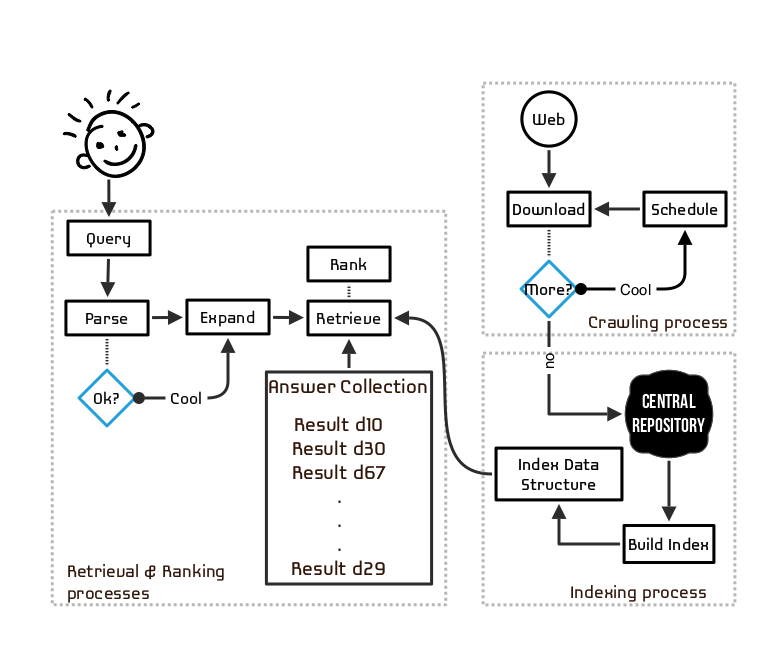
\includegraphics[width=\textwidth]{images/csarchitecture}
    \caption{High level architecture of a code search engine.}
    \label{fig:irarchitecture}
\end{figure}
\pagebreak

\item In addition to the above user and lab studies, a new user study will be conducted comparing \uppercase{SnipR} to a general Web code search engine (e.g., Koders) and an example-centric programming tool that enhances a search interface (e.g., SnipMatch or Blueprint). This study attempts to examine how quickly developers perform a more complete code search task (with or without \uppercase{SnipR}), the quality of the solutions obtained, and the number of queries issued. This study will be based on the subjects trying to solve a programming problem by doing code search. The subjects will be asked not to write any code from scratch, but to instead find example code that best matches the problem at hand. A Latin Square design will be used to control the order in which the search interfaces are presented to subjects at the beginning of the experiment. The data gathered from this study will be used to gauge how efficient the \uppercase{SnipR} approach is in comparison to general and/or code-centric search engines (RQ4).     
\end{itemize}

\fancybreak{\pfbreakdisplay}

\section{Timeline}
\label{sec:workplan}

I expect to take approximately two years to finish from this point. I am 
focusing on the opportunities and challenges outlined in this document. 
Meanwhile, I continue to refine my thesis proposal, and get feedback from other 
researchers. 

\begin{itemize}
\item Winter 2013 - Fall 2014. The first year will focus on stretching 
    \uppercase{SnipR} into an efficient practice.
    \subitem Flesh out command line language (refining and describing all 
    commands in detail).
    \subitem Flesh out system architecture (refining and describing all 
    components in detail).
    \subitem Flesh out \uppercase{SnipR}, the learning algorithm for mapping-based transformations,  
	 the algorithm for applying these mappings, and code retargeting operators.  
    \subitem Write up several position papers on \uppercase{SnipR} using the above discoveries.
    \subitem Implement and integrate the system.
\item Winter 2014 - Fall 2015. The second year will focus on architectural 
    experimentation, evolving the system, and generalizing this work's 
    contributions; including the writing of my dissertation.
    \subitem Write up the initial results product of system integration and 
    architecture.
    \subitem Carry out user experiments; including the evaluation of all \uppercase{SnipR}'s algorithms.
    \subitem Perform a final literature review. 
    \subitem Produce a detailed thesis outline conditioned on experimental 
    results.
    \subitem Finish writing and defend.
\end{itemize}

\chapter{Practical Applications}{}
\label{sec:applications}

\lettrine[lraise=0.1, nindent=0em, slope=-.5em]{T} {HERE ARE MANY} possible practical applications of a \uppercase{SnipR}--aware code search engine. First, the \uppercase{SnipR} approach can be applied throughout many of the phases of the software development process---in or out of the IDEs---and much more:

\begin{itemize}
\item During concept development, to rapidly explore all kinds application 
    scenarios.
\item During prototyping where there is not enough time to invest in 
    code robustness and maintainability~\cite{Brandt:2008wi, Ncube:2008fm, Brandt:2009jb}. 
\item During application refinement using agile development methods. 
\item During program comprehension where the goal is to learn how to program or 
    to teach someone's children how to program.  
\item During code competitions where the emphasis is on speed and time to win 
    the competition\footnote{http://code.google.com/codejam}.
\item During training for a programming interview where the chief goal is succeeding on the 
    interview and possible getting hired.
\end{itemize}

In a world where the vast majority of programming knowledge is archived and curated by millions of ``experts,'' it is not far-fetched to believe that a new category of ``Just in time programmers''\footnote{those ones with the ability to combine snippets to build solutions that will just meet their needs} will arise. Consequently, it is envisioned that the \uppercase{SnipR} approach will be one of the tools that these programmers will use.
\chapter{Conclusion}{}
\label{sec:conclusion}

\lettrine[lraise=0.1, nindent=0em, slope=-.5em]{T}{HIS DOCUMENT HAS} introduced \uppercase{SnipR}, an approach that complements code search with code retargeting capabilities. Unlike prior work, the \uppercase{SnipR} enables developers to engage in a virtuous loop where they find and select only the promising example code that can be retargeted. This will minimize the number of iterations in the search process the developer has to go through, since the evaluation step is only dealing with best choices---choices that would be easier to consume later in the IDE. It is envisioned that \uppercase{SnipR} will not be seen as a competitor to any code search systems, but more like a platform. A platform for searching for suitable code.

\todos
\bibliographystyle{abbrv}
\bibliography{proposal}

\end{document}